\documentclass{whiteboard}
\begin{document}
\begin{frame}[plain,t]
\bbcover{Grafos}{Algoritmo de Floyd-Warshall}{Prof. Edson Alves}{Faculdade UnB Gama}

\end{frame}
\begin{frame}[plain,t]
\begin{tikzpicture}
\node[draw,opacity=0] at (0, 0) {x};
\node[draw,opacity=0] at (14, 8) {x};

	\node[] (floyd) at (2.0, 5.0) { \includegraphics[scale=0.4]{figs/floyd.jpg} };

	\node[] (fname) at (2.0, 2.75) { \bbbold{Robert W. Floyd} };

	\node[] (fdate) at (2.0, 2.25) { \bbtext{(1962)} };


\end{tikzpicture}
\end{frame}
\begin{frame}[plain,t]
\begin{tikzpicture}
\node[draw,opacity=0] at (0, 0) {x};
\node[draw,opacity=0] at (14, 8) {x};

	\node[] (floyd) at (2.0, 5.0) { \includegraphics[scale=0.4]{figs/floyd.jpg} };

	\node[] (fname) at (2.0, 2.75) { \bbbold{Robert W. Floyd} };

	\node[] (fdate) at (2.0, 2.25) { \bbtext{(1962)} };



	\node[] (warshall) at (8.0, 6.0) { \includegraphics[scale=2.4]{figs/warshall.jpg} };

	\node[] (wname) at (11.0, 6.5) { \bbbold{Stephen Warshall} };

	\node[] (wdate) at (11.0, 6.0) { \bbtext{(1962)} };

\end{tikzpicture}
\end{frame}
\begin{frame}[plain,t]
\begin{tikzpicture}
\node[draw,opacity=0] at (0, 0) {x};
\node[draw,opacity=0] at (14, 8) {x};

	\node[] (floyd) at (2.0, 5.0) { \includegraphics[scale=0.4]{figs/floyd.jpg} };

	\node[] (fname) at (2.0, 2.75) { \bbbold{Robert W. Floyd} };

	\node[] (fdate) at (2.0, 2.25) { \bbtext{(1962)} };



	\node[] (warshall) at (8.0, 6.0) { \includegraphics[scale=2.4]{figs/warshall.jpg} };

	\node[] (wname) at (11.0, 6.5) { \bbbold{Stephen Warshall} };

	\node[] (wdate) at (11.0, 6.0) { \bbtext{(1962)} };


	\node[] (roy) at (8.0, 2.0) { \includegraphics[scale=0.1]{figs/roy.jpg} };

	\node[] (rname) at (11.5, 2.5) { \bbbold{Bernard Roy} };

	\node[] (rdate) at (11.5, 2.0) { \bbtext{(1959)} };


\end{tikzpicture}
\end{frame}
\begin{frame}[plain,t]
\begin{tikzpicture}
\node[draw,opacity=0] at (0, 0) {x};
\node[draw,opacity=0] at (14, 8) {x};

	\node[anchor=west] (title) at (0.0, 7.0) { \Large \bbbold{Características do algoritmo de Bellman-Ford} };
\end{tikzpicture}
\end{frame}
\begin{frame}[plain,t]
\begin{tikzpicture}
\node[draw,opacity=0] at (0, 0) {x};
\node[draw,opacity=0] at (14, 8) {x};

	\node[anchor=west] (title) at (0.0, 7.0) { \Large \bbbold{Características do algoritmo de Bellman-Ford} };

	\node[anchor=west] (a) at (0.5, 6.0) { $\star$ \bbtext{Computa o caminho mínimo entre todos os pares de vértices de $G(V, E)$} };

\end{tikzpicture}
\end{frame}
\begin{frame}[plain,t]
\begin{tikzpicture}
\node[draw,opacity=0] at (0, 0) {x};
\node[draw,opacity=0] at (14, 8) {x};

	\node[anchor=west] (title) at (0.0, 7.0) { \Large \bbbold{Características do algoritmo de Bellman-Ford} };

	\node[anchor=west] (a) at (0.5, 6.0) { $\star$ \bbtext{Computa o caminho mínimo entre todos os pares de vértices de $G(V, E)$} };


	\node[anchor=west] (b) at (0.5, 5.0) { $\star$ \bbtext{É capaz de processar arestas negativas} };

\end{tikzpicture}
\end{frame}
\begin{frame}[plain,t]
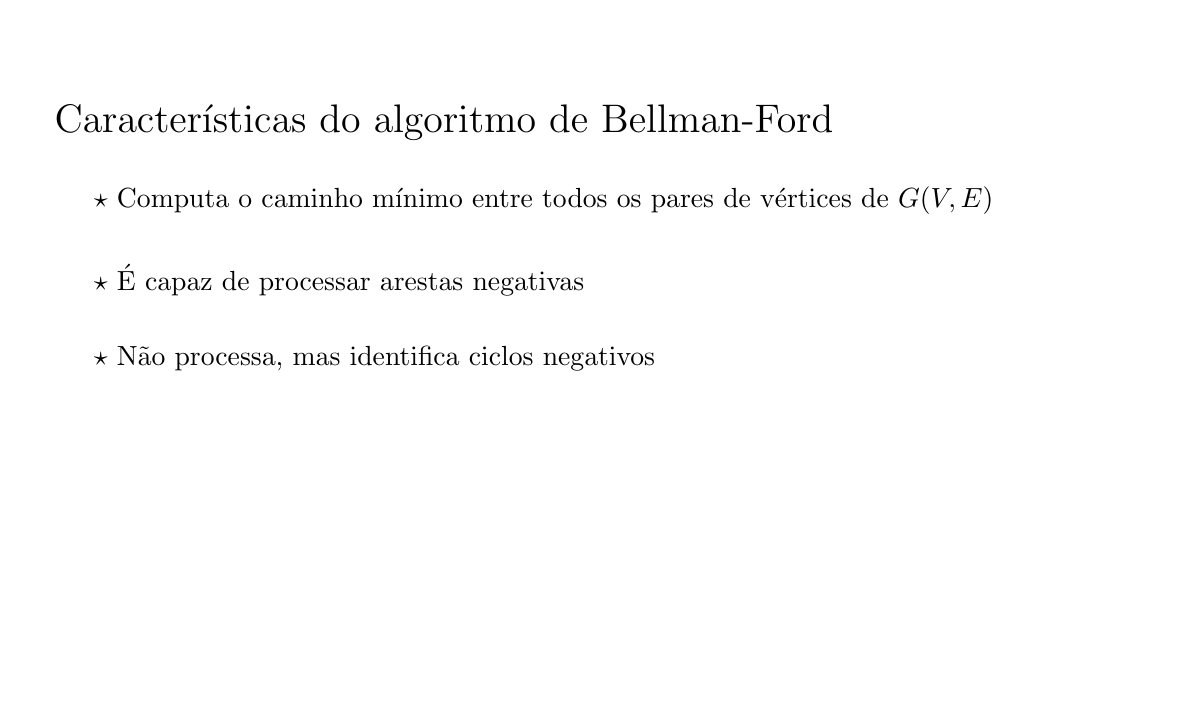
\begin{tikzpicture}
\node[draw,opacity=0] at (0, 0) {x};
\node[draw,opacity=0] at (14, 8) {x};

	\node[anchor=west] (title) at (0.0, 7.0) { \Large \bbbold{Características do algoritmo de Bellman-Ford} };

	\node[anchor=west] (a) at (0.5, 6.0) { $\star$ \bbtext{Computa o caminho mínimo entre todos os pares de vértices de $G(V, E)$} };


	\node[anchor=west] (b) at (0.5, 5.0) { $\star$ \bbtext{É capaz de processar arestas negativas} };


	\node[anchor=west] (c) at (0.5, 4.0) { $\star$ \bbtext{Não processa, mas identifica ciclos negativos} };

\end{tikzpicture}
\end{frame}
\begin{frame}[plain,t]
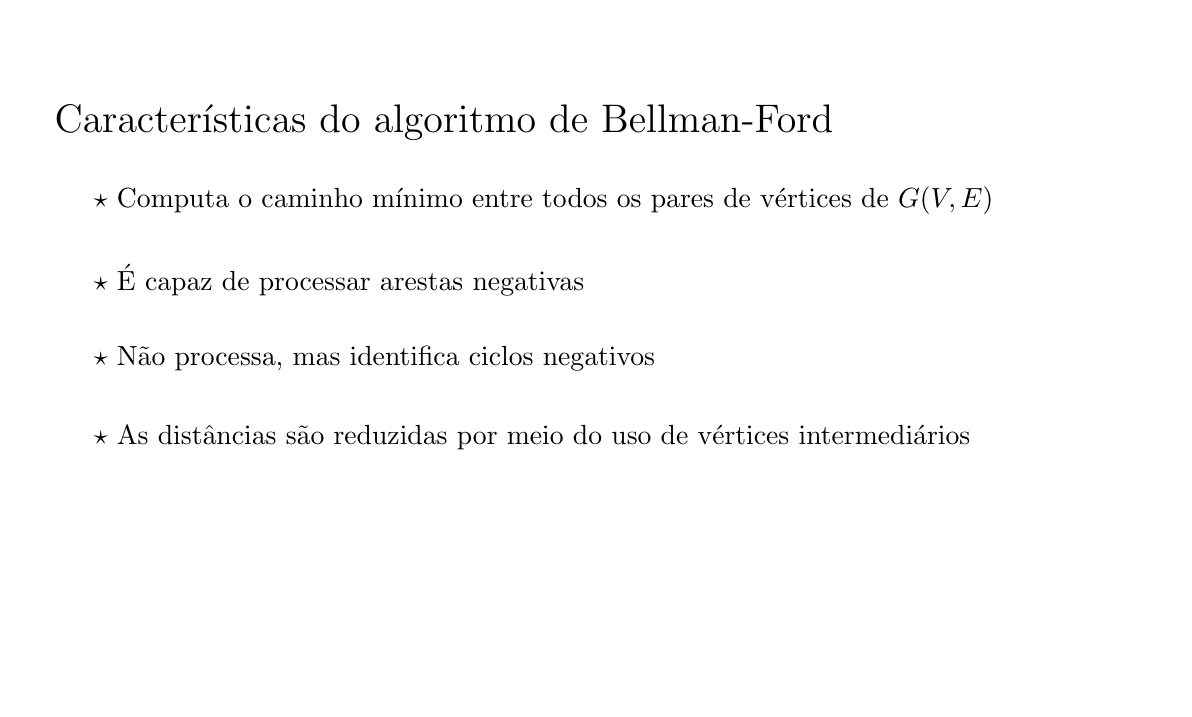
\begin{tikzpicture}
\node[draw,opacity=0] at (0, 0) {x};
\node[draw,opacity=0] at (14, 8) {x};

	\node[anchor=west] (title) at (0.0, 7.0) { \Large \bbbold{Características do algoritmo de Bellman-Ford} };

	\node[anchor=west] (a) at (0.5, 6.0) { $\star$ \bbtext{Computa o caminho mínimo entre todos os pares de vértices de $G(V, E)$} };


	\node[anchor=west] (b) at (0.5, 5.0) { $\star$ \bbtext{É capaz de processar arestas negativas} };


	\node[anchor=west] (c) at (0.5, 4.0) { $\star$ \bbtext{Não processa, mas identifica ciclos negativos} };


	\node[anchor=west] (d) at (0.5, 3.0) { $\star$ \bbtext{As distâncias são reduzidas por meio do uso de vértices intermediários} };

\end{tikzpicture}
\end{frame}
\begin{frame}[plain,t]
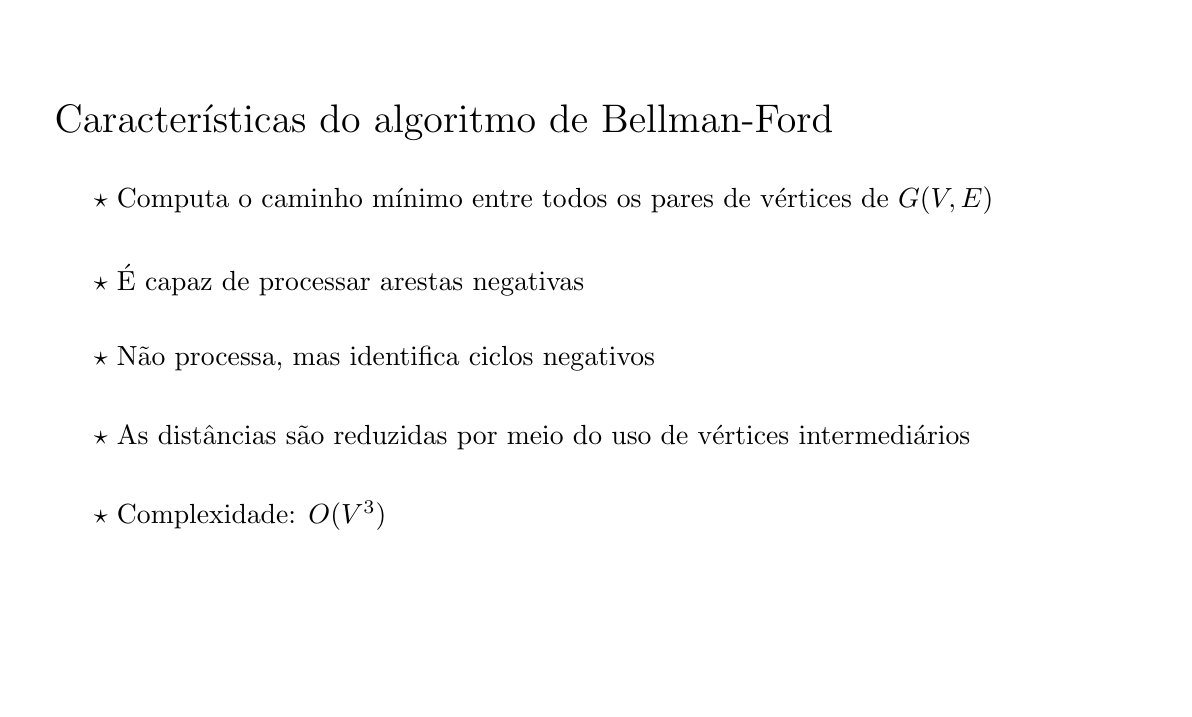
\begin{tikzpicture}
\node[draw,opacity=0] at (0, 0) {x};
\node[draw,opacity=0] at (14, 8) {x};

	\node[anchor=west] (title) at (0.0, 7.0) { \Large \bbbold{Características do algoritmo de Bellman-Ford} };

	\node[anchor=west] (a) at (0.5, 6.0) { $\star$ \bbtext{Computa o caminho mínimo entre todos os pares de vértices de $G(V, E)$} };


	\node[anchor=west] (b) at (0.5, 5.0) { $\star$ \bbtext{É capaz de processar arestas negativas} };


	\node[anchor=west] (c) at (0.5, 4.0) { $\star$ \bbtext{Não processa, mas identifica ciclos negativos} };


	\node[anchor=west] (d) at (0.5, 3.0) { $\star$ \bbtext{As distâncias são reduzidas por meio do uso de vértices intermediários} };


	\node[anchor=west] (e) at (0.5, 2.0) { $\star$ \bbtext{\bbbold{Complexidade}: $O(V^3)$ } };

\end{tikzpicture}
\end{frame}
\begin{frame}[plain,t]
\begin{tikzpicture}
\node[draw,opacity=0] at (0, 0) {x};
\node[draw,opacity=0] at (14, 8) {x};

	\node[anchor=west] (title) at (0.0, 7.0) { \Large \bbbold{Pseudocódigo} };

\end{tikzpicture}
\end{frame}
\begin{frame}[plain,t]
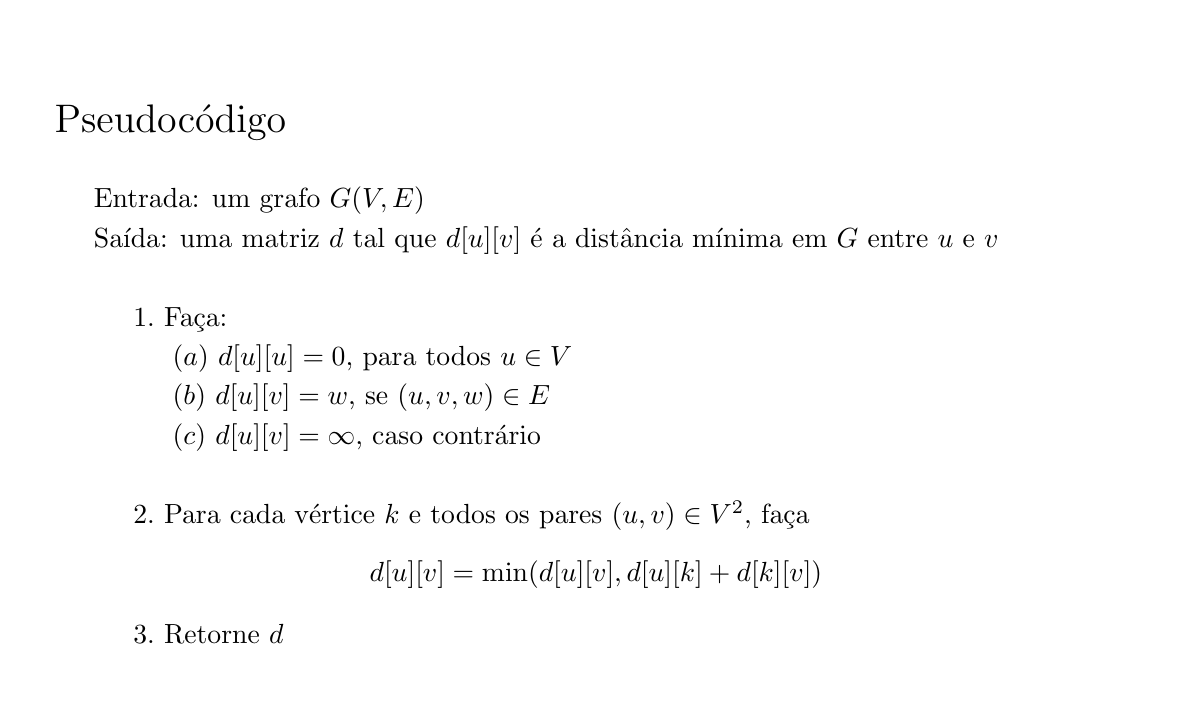
\begin{tikzpicture}
\node[draw,opacity=0] at (0, 0) {x};
\node[draw,opacity=0] at (14, 8) {x};

	\node[anchor=west] (title) at (0.0, 7.0) { \Large \bbbold{Pseudocódigo} };


	\node[anchor=west] (input) at (0.5, 6.0) { \bbemph{Entrada:} \bbtext{um grafo $G(V, E)$} };

	\node[anchor=west] (output) at (0.5, 5.5) { \bbemph{Saída:} \bbtext{uma matriz $d$ tal que $d[u][v]$ é a distância mínima em $G$ entre $u$ e $v$} };

	\node[anchor=west] (step1) at (1.0, 4.5) { $1.$ \bbtext{Faça:} };

	\node[anchor=west] (step1_1) at (1.5, 4.0) { $(a)$ $d[u][u] = 0$, \bbtext{para todos} $u\in V$ };

	\node[anchor=west] (step1_2) at (1.5, 3.5) { $(b)$ $d[u][v] = w$, \bbtext{se} $(u, v, w)\in E$ };

	\node[anchor=west] (step1_3) at (1.5, 3.0) { $(c)$ $d[u][v] = \infty$, \bbtext{caso contrário} };

	\node[anchor=west] (step2) at (1.0, 2.0) { $2.$ \bbtext{Para cada vértice $k$ e todos os pares $(u,v)\in V^2$, faça} };

	\node[] (dist) at (7.0, 1.25) { $d[u][v] = \min(d[u][v], d[u][k] + d[k][v])$ };

	\node[anchor=west] (step3) at (1.0, 0.5) { $3.$ \bbtext{Retorne} $d$ };

\end{tikzpicture}
\end{frame}
\begin{frame}[plain,t]
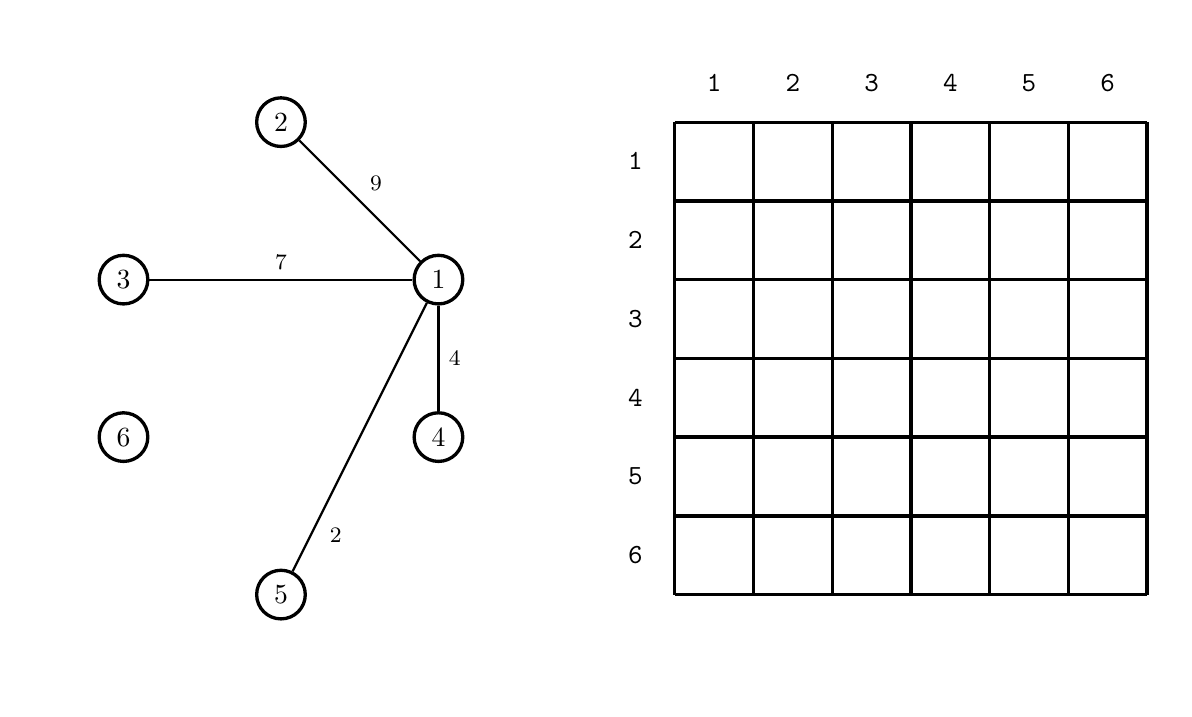
\begin{tikzpicture}
\node[draw,opacity=0] at (0, 0) {x};
\node[draw,opacity=0] at (14, 8) {x};

	\draw[very thick] (8.0, 1.0) grid  (14.0, 7.0);

	\node[] (x1) at (8.5, 7.5) { \bbtext{\tt 1} };

	\node[] (x2) at (9.5, 7.5) { \bbtext{\tt 2} };

	\node[] (x3) at (10.5, 7.5) { \bbtext{\tt 3} };

	\node[] (x4) at (11.5, 7.5) { \bbtext{\tt 4} };

	\node[] (x5) at (12.5, 7.5) { \bbtext{\tt 5} };

	\node[] (x6) at (13.5, 7.5) { \bbtext{\tt 6} };

	\node[] (y1) at (7.5, 6.5) { \bbtext{\tt 1} };

	\node[] (y2) at (7.5, 5.5) { \bbtext{\tt 2} };

	\node[] (y3) at (7.5, 4.5) { \bbtext{\tt 3} };

	\node[] (y4) at (7.5, 3.5) { \bbtext{\tt 4} };

	\node[] (y5) at (7.5, 2.5) { \bbtext{\tt 5} };

	\node[] (y6) at (7.5, 1.5) { \bbtext{\tt 6} };

	\node[very thick,draw,circle] (node1) at (5.0, 5.0) { \bbtext{1} };

	\node[very thick,draw,circle] (node2) at (3.0, 7.0) { \bbtext{2} };

	\node[very thick,draw,circle] (node3) at (1.0, 5.0) { \bbtext{3} };

	\node[very thick,draw,circle] (node4) at (5.0, 3.0) { \bbtext{4} };

	\node[very thick,draw,circle] (node5) at (3.0, 1.0) { \bbtext{5} };

	\node[very thick,draw,circle] (node6) at (1.0, 3.0) { \bbtext{6} };

	\draw[thick](node1) to node[above right] {\footnotesize \bbinfo{9}} (node2);

	\draw[thick](node1) to node[above] {\footnotesize \bbinfo{7}} (node3);

	\draw[thick](node1) to node[right] {\footnotesize \bbinfo{4}} (node4);

	\draw[thick](node1) to node[below right,pos=.8] {\footnotesize \bbinfo{2}} (node5);



\end{tikzpicture}
\end{frame}
\begin{frame}[plain,t]

\end{frame}
\end{document}
